\documentclass[aspectratio=169,usenames,dvipsnames]{beamer}
\usepackage{graphicx}
\usepackage{multimedia}
\usepackage{media9}
\usepackage{url}
\usepackage[algoruled,vlined,linesnumbered]{algorithm2e}
%\usepackage{amsmath}
%\usepackage{amssymb}
\usepackage{latexsym}
\usepackage{multirow}
\usepackage{comment}
\usepackage{wasysym}
\usepackage{units}
\usepackage{wrapfig}
\usepackage{extarrows}
\usepackage{diagbox}
\usepackage{qtree}
\usepackage{booktabs}

%%%%%%%%%%%% My packages %%%%%%%%%%%%%%%%%%%%%%%%%%%%
\usepackage[symbol]{footmisc}
\usepackage{booktabs}

%\usepackage{longtable}
%\usepackage{float}
%\usepackage{colortbl}
%\usepackage{threeparttable}
%\usepackage{tabu}

\usepackage{MnSymbol}

% bibliography
\usepackage[backend=bibtex,style=authoryear]{biblatex}
\addbibresource{bibliography0.bib}

% define slide theme
%\usetheme{Boadilla}
\usetheme{default}

% MATLAB colors: https://www.mathworks.com/help/matlab/ref/matlab.graphics.chart.primitive.histogram-properties.html
\definecolor{m1}{rgb}{0,0.4470,0.7410}
\definecolor{m2}{rgb}{0.8500,0.3250,0.0980}
\definecolor{m3}{rgb}{0.9290,0.6940,0.1250}
\definecolor{m4}{rgb}{0.4940,0.1840,0.5560}
\definecolor{m5}{rgb}{0.4660,0.6740,0.1880}
\definecolor{m6}{rgb}{0.3010,0.7450,0.9330}
\definecolor{m7}{rgb}{0.6350,0.0780,0.1840}

\newcommand{\tcb}[1]{\textcolor{m1}{#1}}
\newcommand{\tco}[1]{\textcolor{m2}{#1}}
\newcommand{\tcv}[1]{\textcolor{m4}{#1}}
\newcommand{\tcg}[1]{\textcolor{m5}{#1}}
\newcommand{\tcm}[1]{\textcolor{m7}{#1}}

% define the heading color
\definecolor{myorange}{rgb}{0.807,0.3137,0.047}
\makeatletter
\colorlet{beamer@blendedblue}{myorange}
\makeatother

\definecolor{gray75}{gray}{0.75}

% define the footer
\definecolor{gray50}{gray}{0.5}
\setbeamertemplate{footline}[text line]{%
\parbox{\linewidth}{\vspace*{-8pt}\textcolor{gray50}{\inserttitle\hfill\insertpagenumber}}}

% get rid of the navigations symbols at the bottom
\setbeamertemplate{navigation symbols}{}

% custom font
%\usepackage{heuristica}
%\usepackage[heuristica,vvarbb,bigdelims]{newtxmath}
%\usepackage[T1]{fontenc}
%\renewcommand*\oldstylenums[1]{\textosf{#1}}
% More fonts here: http://www.tug.dk/FontCatalogue/mathfonts.html

%\usepackage[default]{comfortaa}
%\usepackage[T1]{fontenc}

\usepackage[sfdefault,light]{roboto}  
\usepackage[T1]{fontenc}


%%%%%%%%%%%%% Vadim's macro definitions %%%%%%%%%%%%%%%%%%

\newtheorem{df}{Definition}
\newtheorem{notation}{Notation}
\newtheorem{col}{Corollary}
\newtheorem{lem}{Lemma}

\newcommand{\td}{\,\nicefrac{\times}{\div}\,}

\newcommand{\bt}{\begin{theorem}\em}
\newcommand{\et}{\end{theorem}}
\newcommand{\Qed}{$\blacksquare$}
\renewcommand{\nin}{\noindent}
\newcommand{\bea}{\begin{eqnarray}}
\newcommand{\eea}{\end{eqnarray}}
\newcommand{\bdf}{\begin{df}\em}
\newcommand{\edf}{\end{df}}

\newcommand{\ben}{\begin{enumerate}}
\newcommand{\een}{\end{enumerate}}
\newcommand{\bei}{\begin{itemize}}
\newcommand{\eei}{\end{itemize}}
\newcommand{\ie}{\item}

\newcommand{\midb}{\pmb{\mid}}

\newcommand{\dist}{\operatorname{dist}}
\newcommand{\avg}{\operatornamewithlimits{avg}\limits}
\renewcommand{\arg}{\operatornamewithlimits{arg}\limits}
\newcommand{\round}{\operatorname{round}}
\newcommand{\lop}{\operatorname{lop}}
%\renewcommand{\min}{\operatornamewithlimits{argmin}\limits}
\renewcommand{\max}{\operatornamewithlimits{max}\limits}
\newcommand{\median}{\operatornamewithlimits{median}\limits}
\newcommand{\mean}{\operatornamewithlimits{mean}\limits}
\newcommand{\argmax}{\operatornamewithlimits{argmax}\limits}
\newcommand{\argmin}{\operatornamewithlimits{argmin}\limits}

\numberwithin{equation}{section}
\numberwithin{theorem}{section}
\numberwithin{lem}{section}
\numberwithin{df}{section}

\newcommand{\citea}[1]
{\citeauthor{#1} (\citeyear{#1})}

\setbeamerfont{caption}{series=\normalfont,size=\fontsize{6}{6}}
\definecolor{gray75}{gray}{0.75}
\setbeamertemplate{caption}{\raggedright\textcolor{myorange}{\insertcaption}\par}

\begin{document}

\title{Core Expansion in Optimization Crosswords}
\author{Adi Botea and Vadim Bulitko}
\institute{Eaton \& University of Alberta} 
%\institute{
\includegraphics[width=0.2\textwidth]{_template/uofa.pdf}} 

\date{July 14, 2023}

\frame{\titlepage} 

%%%%%%%%%%%%%%%%%%%%%%%%%%%%%%%%%%%%%%%%%%%%%%%%%%%%%%%%%%%%%%%%%%%%%%%%%%%%%%%%

\begin{frame}{Outline}

\bei

\ie Problem

\bigskip

\ie Contribution

\bigskip

\ie Approach

\bigskip

\ie Results

\bigskip

\ie Conclusions

\eei

\end{frame}

%%%%%%%%%%%%%%%%%%%%%%%%%%%%%%%%%%%%%%%%%%%%%%%%%%%%%%%%%%%%%%%%%%%%%%%%%%%%%%%%

\begin{frame}{Romanian Crosswords Competition ({\sc Roco})}

\begin{columns}
\column{0.6\linewidth}
\bei
\ie Annual competition: 1965 to present
\bei 
\ie top 12 human-submitted grids published
\eei
\ie AI used to lag behind

\bigskip

\ie Input: word lists
\bei
\ie regular Romanian words (about $134$K)
\ie thematic words, vary per year (e.g., $387$)
\eei

\bigskip

\ie Task:
\bei 
\ie build a $13\times13$ grid filled with words
\bei
\ie some constraints
\eei
\ie score = sum of lengths of all thematic words
\eei

\eei

\column{0.4\linewidth}
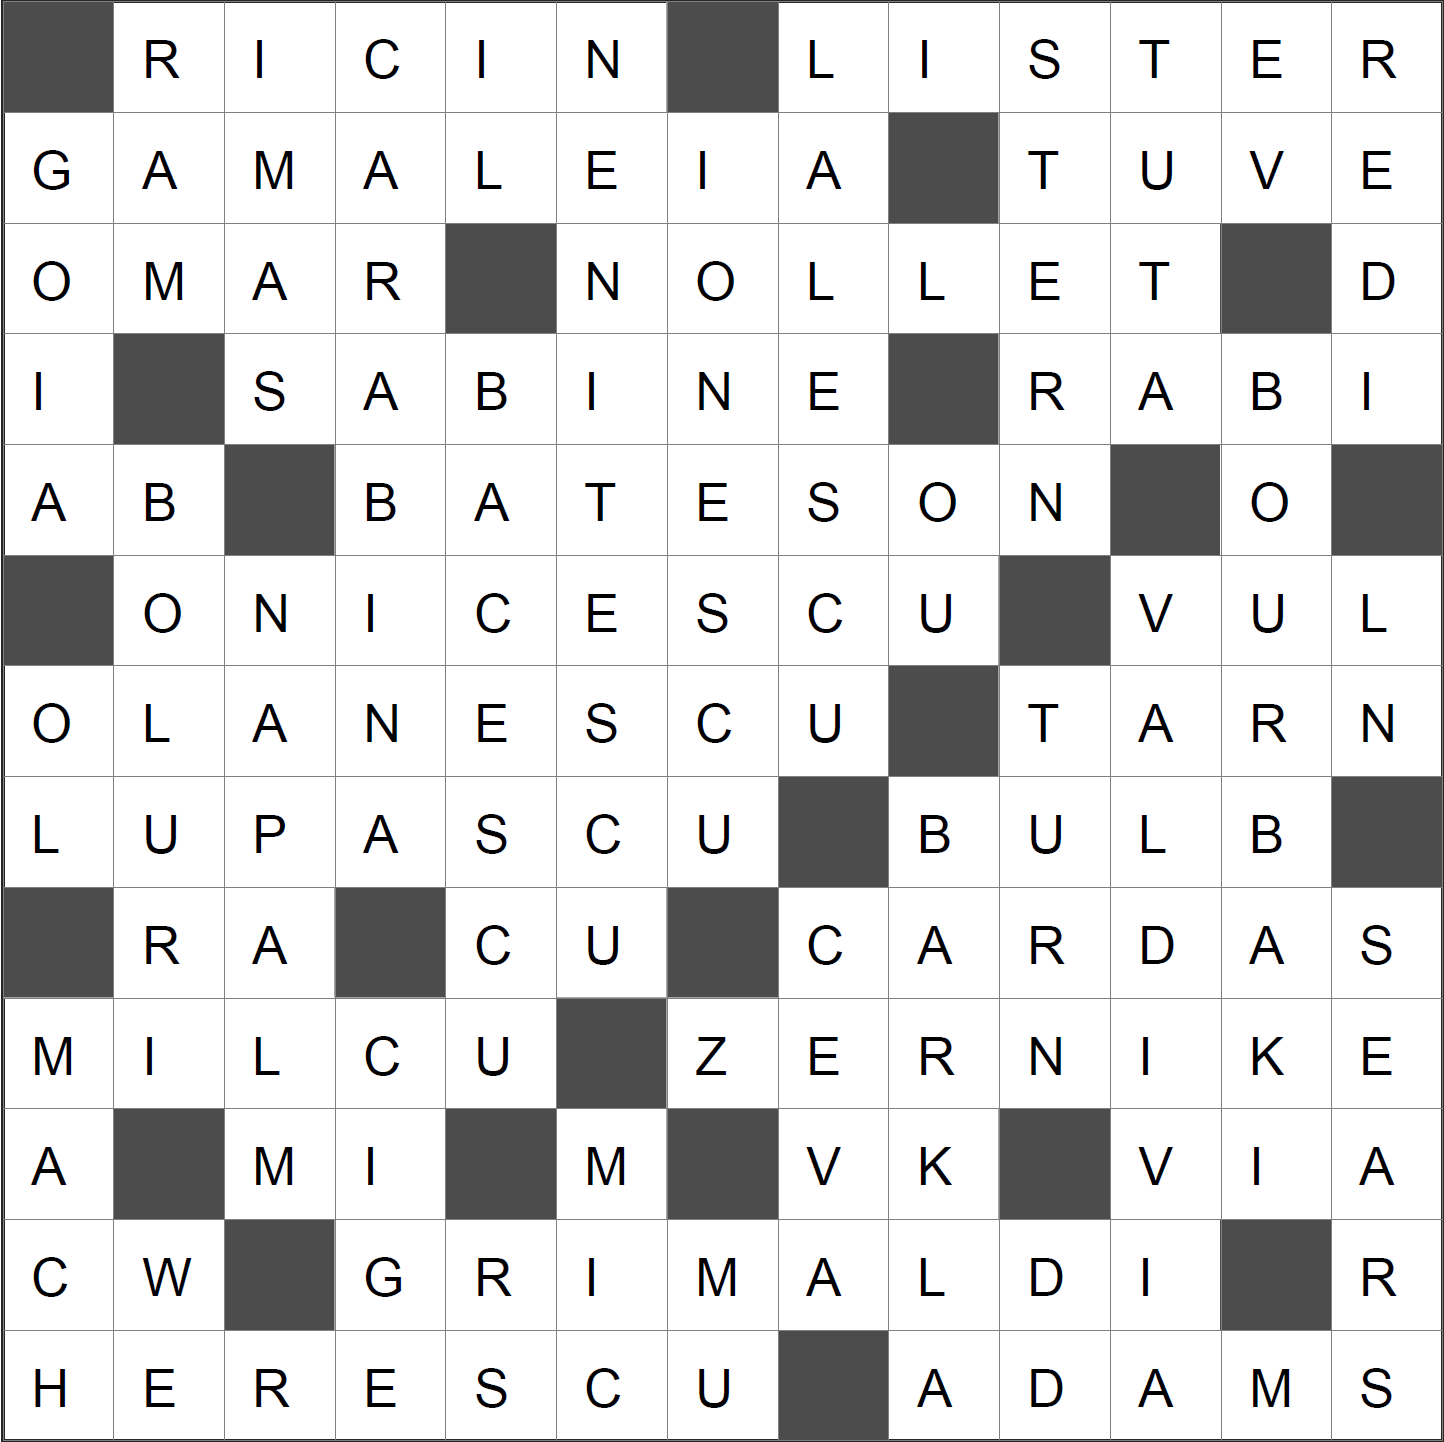
\includegraphics[width=\columnwidth]{2013b.png}
\end{columns}
\end{frame}

\begin{frame}{Main Contribution}

Breakthrough in bringing the AI performance in the vicinity of human champions

\end{frame}

\begin{frame}{Main Steps}

\begin{columns}
\column{0.7\linewidth}
\bei
\ie Build cores from a \emph{pattern} taken as input
\ie Build expanded cores
\ie Build seeds
\ie Evolve seeds into full solutions
\eei
\column{.3\linewidth}
\centering
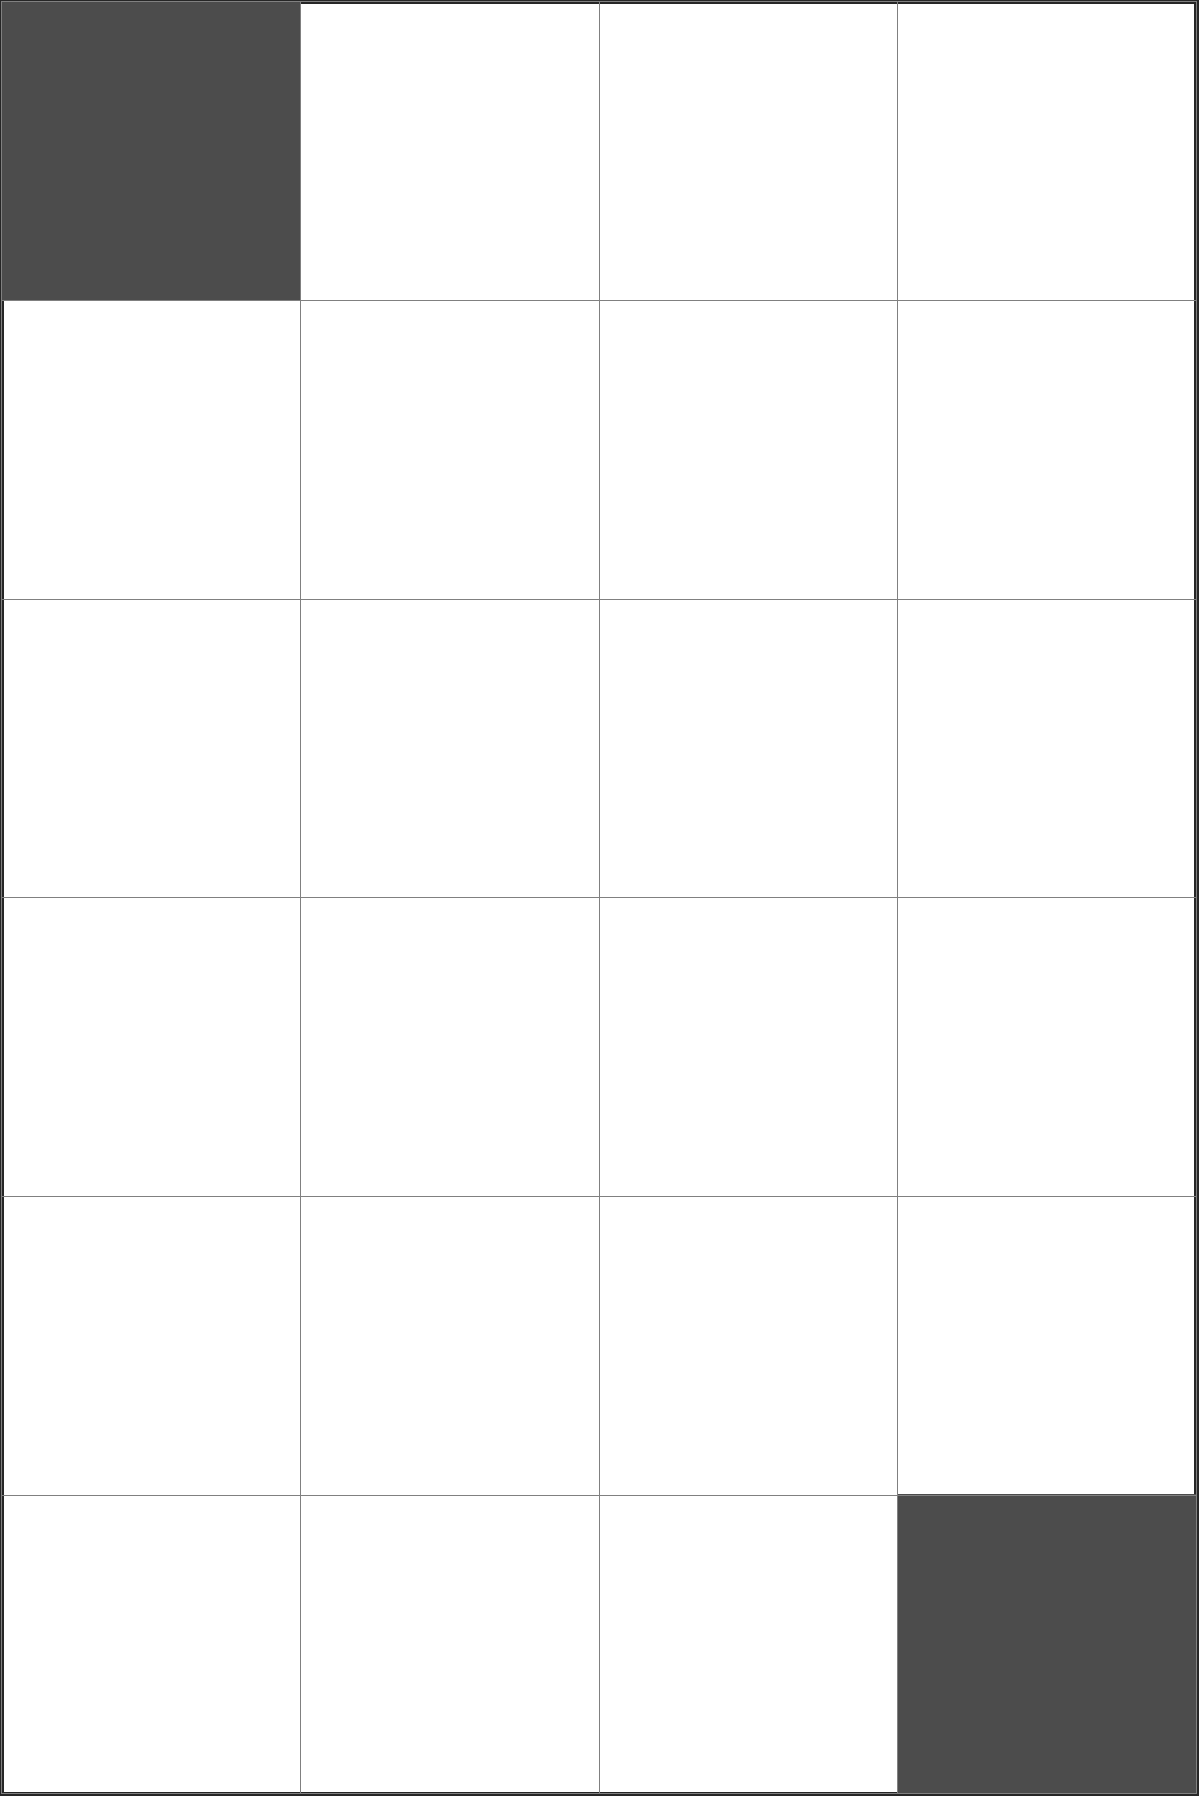
\includegraphics[height=3cm]{_plots/6x4-puzzle.png}\\
A pattern is a rectangular grid with no letters.
\end{columns}

\end{frame}


\begin{frame}{Cores}

\begin{columns}
\column{0.7\linewidth}
\begin{block}{Definition}
A \emph{core} is a pattern filled with letters. We require that each ``word'' in a core is a substring of a thematic word.
\end{block}
\begin{block}{Building cores from a pattern}
\bei
\ie Construct a small puzzle
\bei 
\ie The grid is the pattern
\ie The dictionary contains substrings of thematic words
\eei
\ie Feed puzzle into {\sc Wombat} and generate multiple solutions
\eei
\end{block}
\column{.3\linewidth}
\centering
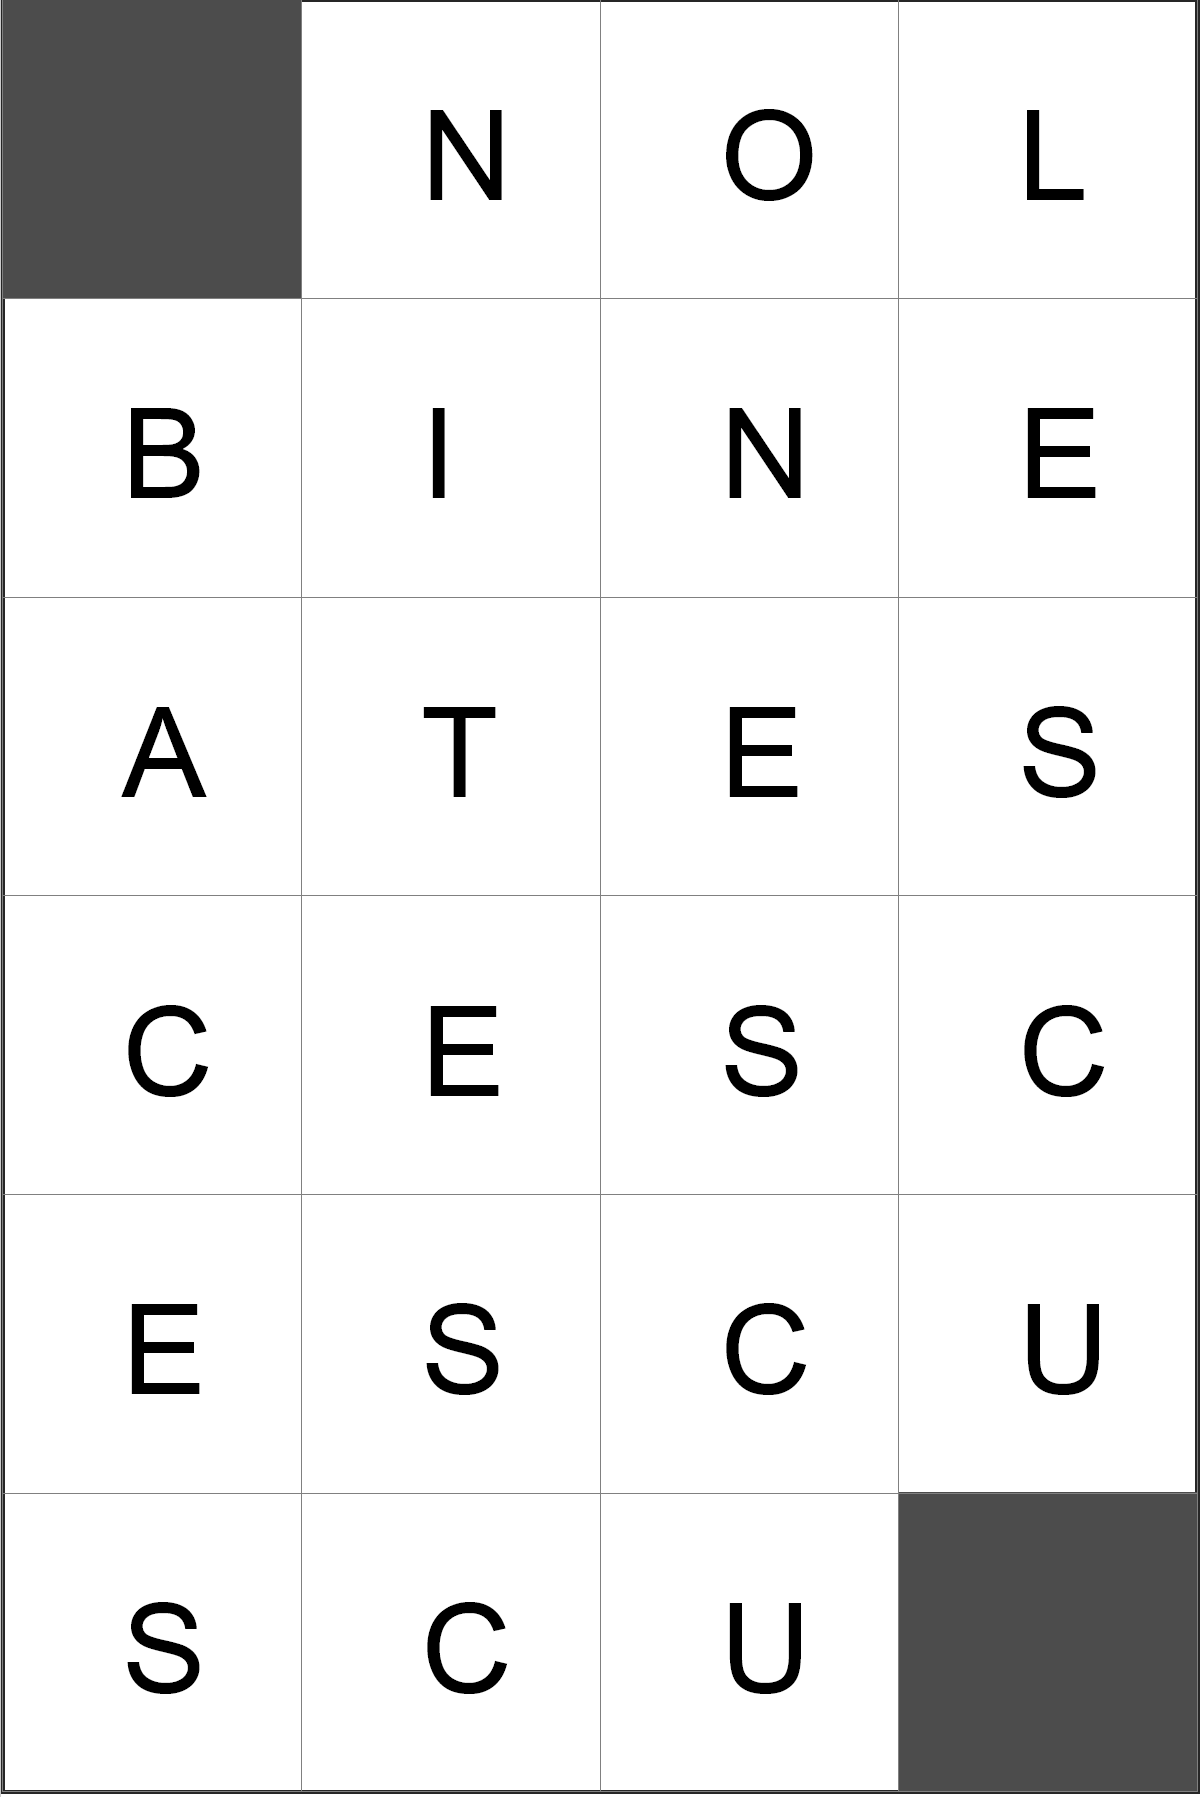
\includegraphics[height=3cm]{_plots/core-6x4-puzzle.png}
\end{columns}

\end{frame}

\begin{frame}{Expanded Cores}

\begin{columns}
\column{0.5\linewidth}
\begin{block}{Definition}
An \emph{expanded core} is a rectangular grid with white cells, black cells, and white cells with letters.
It contains full thematic words, with black cells by each endpoint.
\end{block}
\begin{block}{Building expanded cores from a core}
\bei
\ie Match full thematic words over strings in the core
\ie Depth first search
\eei
\end{block}
\column{.5\linewidth}
\centering
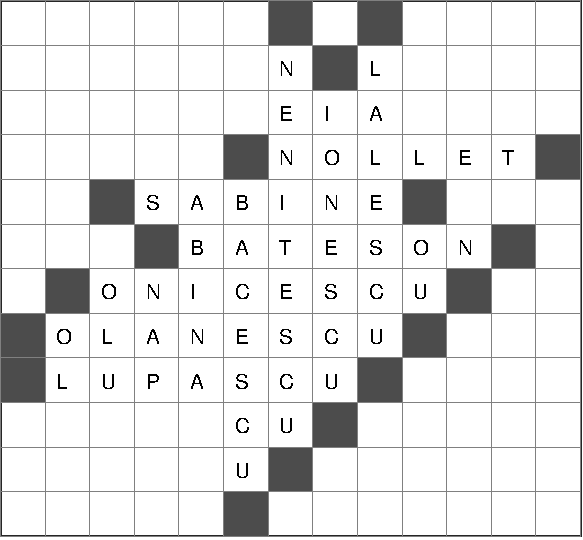
\includegraphics[height=6cm]{_plots/extcore-alive-0-puzzle-72-2975-1488--1--1.pdf}
\end{columns}

\end{frame}


\begin{frame}{Seeds}

\begin{columns}
\column{0.5\linewidth}
\begin{block}{Definition}
A \emph{seed} is a full-size $13\times13$ grid with white cells, black cells, and white cells with letters.
\end{block}
\begin{block}{Building seeds from an expanded core}
\bei
\ie Place the expanded core inside the $13\times13$ grid
\ie Shift horizontally and vertically to obtain multiple seeds
\ie Prune away seeds proven illegal
\eei
\end{block}
\column{.5\linewidth}
\centering
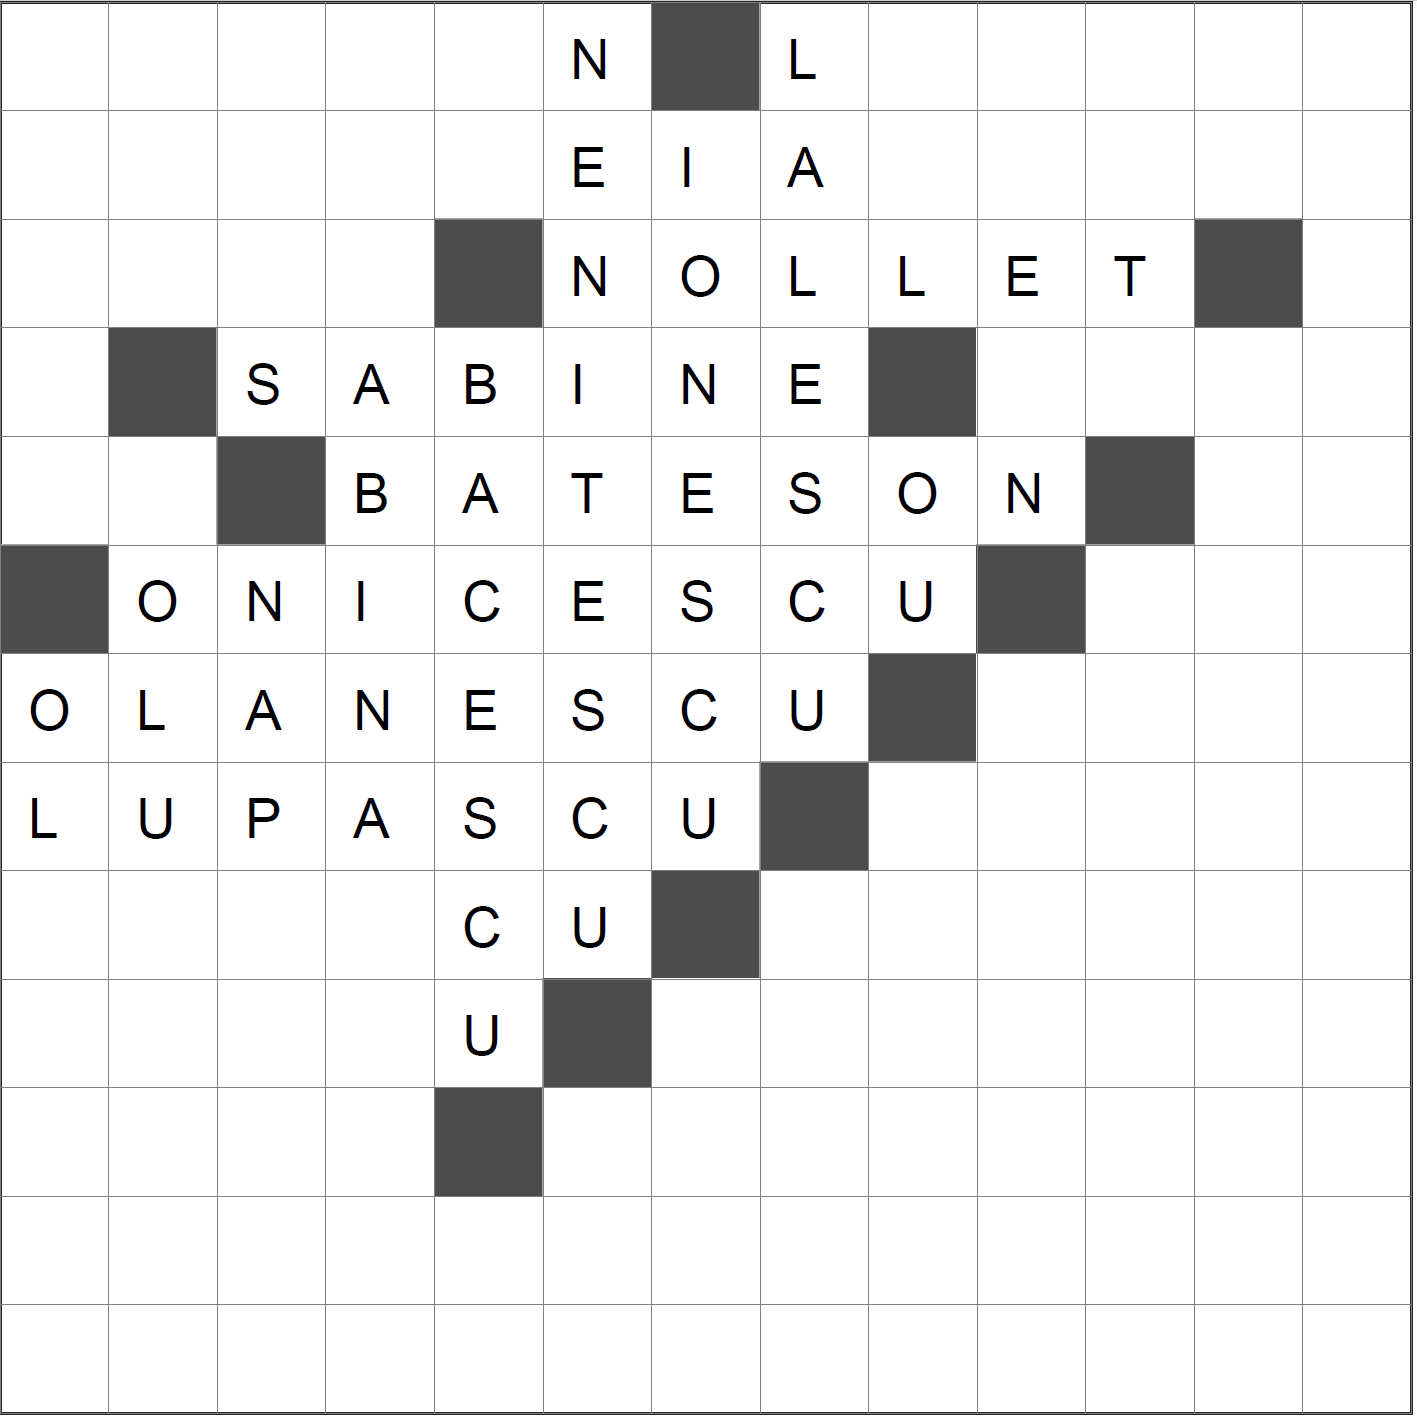
\includegraphics[height=6cm]{_plots/alive-0-puzzle-72-2975-1488--1--1.png} \hspace{1cm}
\end{columns}

\end{frame}

\begin{frame}{Example with Building a Seed}

\begin{figure}
\centering
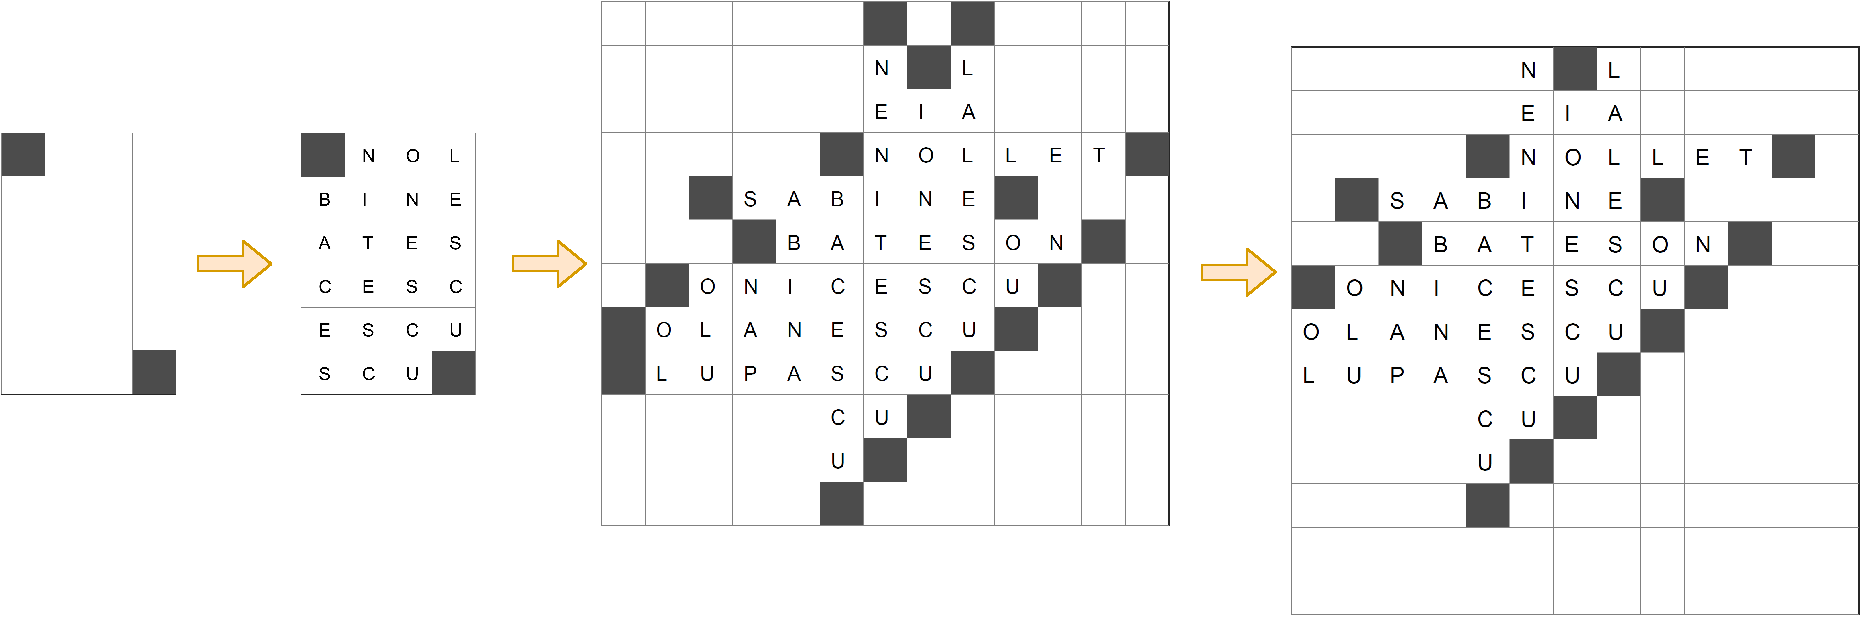
\includegraphics[width=\textwidth]{figs/4part.pdf}
\caption{Gradually building a seed: pattern $\rightarrow$ core $\rightarrow$ expanded core $\rightarrow$ seed. The different stages of the build are aligned vertically to illustrate how the expansion and build happen. Note, for instance, how the partial word ``NOL'' becomes ``NOLLET''. }
\label{fig:pattern}
\end{figure}

\end{frame}


%%%%%%%%%%%%%%%%%%%%%%%%%%%%%%%%%%%%%%%%%%%%%%%%%%%%%%%%%%%%%%%%%%%%%%%%%%%%%%%%

%%%%%%%%%%%%%%%%%%%%%%%%%%%%%%%%%%%%%%%%%%%%%%%%%%%%%%%%%%%%%%%%%%%%%%%%%%%%%%%%

%%%%%%%%%%%%%%%%%%%%%%%%%%%%%%%%%%%%%%%%%%%%%%%%%%%%%%%%%%%%%%%%%%%%%%%%%%%%%%%%

%%%%%%%%%%%%%%%%%%%%%%%%%%%%%%%%%%%%%%%%%%%%%%%%%%%%%%%%%%%%%%%%%%%%%%%%%%%%%%%%

\begin{frame}{Conclusions}


\end{frame}

%%%%%%%%%%%%%%%%%%%%%%%%%%%%%%%%%%%%%%%%%%%%%%%%%%%%%%%%%%%%%%%%%%%%%%%%%%%%%%%%



\begin{frame}[allowframebreaks]{Bibliography}
\renewcommand*{\bibfont}{\footnotesize}
\printbibliography
\end{frame}

%%%%%%%%%%%%%%%%%%%%%%%%%%%%%%%%%%%%%%%%%%%%%%%%%%%%%%%%%%%%%%%%%%%%%%%%%%%%%%%%

\end{document}



